%
% ---------------------------------------------------
%
% Trabajo de Final de Grado:
% Author: Gonzalo Jesús García Martín <dracoyue@gmail.com>
% Capítulo: Introducción
% Fichero: Cap4_Herramientas.tex
%
% ----------------------------------------------------
%

\cleardoublepage
\chapter{Herramientas}
\label{chap:tools}

	El software usado en el desarrollo de \CollegeApp\ ha sido el siguiente:
	\begin{itemize}
		\item {\bf AndroidStudio} \cite{1:androidstudio:online}: Entorno de desarrollo integrado oficial para el desarrollo de aplicaciones para {\it Android}, basado en {\it IntelliJ IDEA} \cite{14:intellij:online}.
		Ha sido seleccionado por ser un entorno de programación moderno, de uso intuitivo y ligero en comparación con otros entornos de desarrollo ya existentes como {\it eclipse} \cite{15:eclipse:online} o {\it netbeans} \cite{22:netbeans:online} que son más pesados, ya que soportan más lenguajes de programación.
		\item {\bf Android} \cite{2:android:online}: Sistema operativo basado en el {\it núcleo de Linux} para dispositivos móviles, televisores, automóviles y relojes inteligentes.
		\item {\bf Firebase} \cite{6:firebase:online}: Proveedor de contenidos que proporciona servicios en la nube de forma fácil y segura, con una integración sencilla con las nuevas tecnologías. Ofrece servicios de recuperación y almacenamiento de datos, registro y acceso de usuarios, reglas de seguridad, simulador y análisis de datos entre otros. Los datos almacenados en este servicio no son datos \href{http://es.wikipedia.org/wiki/SQL}{\textit{SQL}}, sino que son datos \href{http://es.wikipedia.org/wiki/JSON}{\textit{JSON}} \cite{7:json:online}. Ha sido elegido por ser uno de los servicios en la nube más sencillos de utilizar.
		Sistemas con los que {\it Firebase} está integrado:
		\begin{itemize}
			\item {\bf Android}: Sistema Operativo para dispositivos móviles propiedad de Google.
			\item {\bf IOS} \cite{16:ios:online}: Sistema operativo para dispositivos móviles propiedad de Apple Inc.
			\item {\bf Servicios Web}.
			\item {\bf Servicios REST} \cite{18:rest:online}: Es un conjunto de principios de arquitectura, pero en la actualidad se usa en el sentido más amplio para describir cualquier interfaz entre sistemas que utilice directamente HTTP \cite{60:http:online} para obtener datos o indicar la ejecución de operaciones sobre los datos, en cualquier formato sin las abstracciones adicionales de los protocolos basados en patrones de intercambio de mensajes, como por ejemplo SOAP \cite{56:soap:online}.
		\end{itemize}
	\end{itemize}
	
	\section{Otros Servicios en la Nube: Parse \cite{16:parse:online}}
	Proveedor de servicios en la nube alternativo a {\it Firebase} que ofrece eventos, autenticación de usuarios, almacenamientos de datos, análisis y {\it notificaciones push} entre otros.
	
	\bigskip
	Tras la implementación de una aplicación ejemplo para valorar {\it Parse}, se ha seleccionado {\it Firebase} por estar diseñado para la construcción de datos en tiempo real. Al acceder a través de una librería cliente los datos se sincronizan en tiempo real rápidamente. También ofrece una {\it interfaz de programación de aplicaciones} \cite{23:api:online}  de seguridad basada en la expresión altamente flexible que permite un control preciso sobre el acceso a los datos de los clientes.
	
	\bigskip
	{\it Parse} está integrado con las siguientes tecnologías:
	\begin{itemize}
		\setlength{\itemsep}{1pt}
		\setlength{\parskip}{0pt}
		\setlength{\parsep}{0pt}
		\item {\it IOS}.
		\item {\it Android} \cite{2:android:online}.
		\item {\it Javascript}.
		\item {\it OSX}.
		\item {\it Unity}: Software para la creación de videojuegos.
		\item {\it PHP}: Lenguaje de programación.
		\item {\it .Net + Xamarin}.
		\item {\it Arduino}: Hardware libre que consiste en una placa con un microcontrolador y un entorno de programación.
		\item {\it Embedded C}: Lenguaje de programción que extiende sus funcionalidades de C.
		\item {\it Servicios REST}.
	\end{itemize}
	
	\subsubsection{Instalación}
	\begin{itemize}
		\item {\bf Descarga}: Descargar librería de {\it Parse}.
		\item {\bf Librería}: Añadir la librería de {\it Parse} en el archivo {\ttfamily build.gradle} que esta dentro de la carpeta {\ttfamily app} en el directorio raíz del proyecto. Véase listado \ref{code:gradleParse}

		\lstinputlisting[float = h!,language=Java,caption={Importación de la librería de {\it Parse}},label={code:gradleParse}]{Code/buildParse.gradle}
		\newpage
		
		\item {\bf Uso}: En los archivos de clase {\ttfamily  .java}\ \cite{19:java:online} seguir los siguientes pasos:
		\begin{itemize}
			\item {\bf Librerías}: Importar las librerías necesarias:
			\begin{itemize}
				\item {\bf Cliente Firebase}: Importar la librería del cliente.
				\item {\bf Consultas}: Importar la librería de consultas ({\ttfamily ParseQuery}).
				\item {\bf Listeners}: Importar la librería de oyentes ({\ttfamily FindCallback}).
				\item {\bf Excepciones}: Importar la librería de excepciones ({\ttfamily ParseException}).
				\item {\bf Objetos}: Importar la librería de objetos ({\ttfamily ParseObject}).
				\item {\bf Usuarios}: Importar la librería de atenticación de usuarios ({\ttfamily ParseUser}).
			\end{itemize}
			\item {\bf Claves}: Crear dos contantes de tipo cadena ({\it String}) en las introduciremos manualmente la identificación de la aplicación ({\it AppID}) y la clave del cliente ({\it CLIENT\_KEY}).
			\item {\bf Contexto}: Añadir el contexto en que se va a usar en la función {\ttfamily onCreate()} con la identificación y la clave.
			\item {\bf Consultas}: Preparar la consulta que se va a hacer.
			\item {\bf Oyentes}:Añadir un oyente ({\it Listener}) a la consulta.
		\end{itemize}
		
		En el listado \ref{code:parse} se presenta un ejemplo de uso de la librería.
		
		\newpage
		\noindent
		\lstinputlisting[language=Java,caption={Ejemplo de uso de {\it Parse} (parte del código)},label={code:parse}]{Code/ParseExample.java}
	\end{itemize}
		
	\section{Instalación de las herramientas usadas}
	En esta sección se procederá a explicar la instalación de {\it AndroidStudio} y {\it Firebase}.
	
	\subsection{AndroidStudio}
	\begin{itemize}
		\item {\bf JDK}: Descargar e instalar {\it Java Development Kit} \cite{17:jdk:online}.
		\item {\bf Descarga}: Descargar {\it AndrodiStudio}.
		\item {\bf Instalación}: Ejecutar el archivo de instalación descargado y seguir los pasos indicados por el instalador.
		\item {\bf SDK}: Añadir paquetes {\it SDK} con el gestor de paquetes ({\it SDK Manager}) seleccionándolo en la barra de herramientas.
		\item {\bf Paquetes}: Seleccionar las versiones de {\it Android} \cite{2:android:online} a instalar, se pueden elegir o quitar paquetes concretos de cada versión. Darle a {\it Install}. Es importante que ademas de instalar las versiones a utilizar, se instalen los siguientes paquetes:
		\begin{itemize}
			\item {\it Android SDK Tools}.
			\item {\it Android SDK Platform-tools}.
			\item {\it Android SDK Build-tools} (La versión más actual).
			\item Extras \textgreater {\it Android Support Repository}.
			\item Extras \textgreater {\it Android Support Library}.
			\item Extras \textgreater {\it Google USB Driver}.
		\end{itemize}
	\end{itemize}
	
	En la figura \ref{fig:SdkManagerPackages} se pueden observar los paquetes que se pueden instalar.
	
	\begin{figure}[h !]
		\centering
		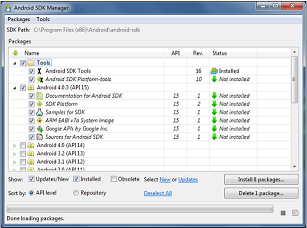
\includegraphics[scale=0.5]{Packages}
		\caption{Paquetes en SDK Manager}
		\label{fig:SdkManagerPackages}
	\end{figure}
	
	\newpage
	\subsection{Firebase}
	\begin{itemize}
		\item {\bf Librería}: Añadir la librería de {\it Firebase} en el archivo {\ttfamily build.gradle} que está dentro de la carpeta {\ttfamily app} en el directorio raíz del proyecto \CollegeApp. En el listado \ref{code:gradle} se puede observar cómo se importa la librería de {\it Firebase}.
		
		\lstinputlisting[float = h!,language=Java,caption={Importación de la librería de {\it Firebase}},label={code:gradle}]{Code/build.gradle}
		
		\item {\bf Uso}: En los archivos de clase {\ttfamily .java }\cite{19:java:online} seguir los siguientes pasos:
		\begin{itemize}
			\item {\bf Librerías}: Se han de importar la librerías necesarias:
			\begin{itemize}
				\item {\bf Cliente Firebase}: Importar la librería del cliente.
				\item {\bf Errores Firebase}: Importar la librería de errores en consultas.
				\item {\bf Datos Firebase}: Importar la librería que permite la devolución de datos desde {\it Firebase}.
				\item {\bf Consultas Firebase}: Importar la librería para consultas.
				\item {\bf Librería Oyentes}: Importar la librería de los oyentes ({\it Listeners}).
			\end{itemize}
			\item {\bf Contexto}: Añadir el contexto en que se va a usar en la función {\ttfamily onCreate()}.
			\item {\bf Referencias}: Añadir una referencia a la base de datos o tabla de la misma a la que se van a hacer las consultas.
			\item {\bf Consultas}: Preparar la consulta que se va a hacer.
			\item {\bf Oyentes}: Añadir un oyente ({\it Listener}) a la consulta.
		\end{itemize}
	\end{itemize}

	En el listado \ref{code:firebase} se presenta un ejemplo del uso de la librería {\it Firebase}.
	
	\lstinputlisting[float = h!,language=Java,caption={Ejemplo de uso de {\it Firebase}},label={code:firebase}]{Code/FirebaseExample.java}
	
	\section{Tutoriales}
	
	Antes de comenzar con el desarrollo de la aplicación propiamente dicha, se han implementado diversas aplicaciones a modo de ejemplo para afianzar los conocimientos sobre {\it Android}.
	
	\begin{enumerate}
		\setlength{\itemsep}{1pt}
		\setlength{\parskip}{0pt}
		\setlength{\parsep}{0pt}
		\item {\it Build your first app} \cite{29:firstapp:online}
		\item {\it Adding the action bar}
		\item {\it Supporting Different Devices} \label{tut:3}
		\item {\it Managing the Activity Lifecycle}
		\item {\it Building a Dynamic UI with Fragments} \label{tut:5}
		\item {\it Saving Data}
		\item {\it Interacting with Other Apps}
		\item {\it Sharing Simple Data}
		\item {\it Sharing Files}
		\item {\it Sharing Files with NFC}
		\item {\it Managing Audio Playback}
		\item {\it Capturing Photos}
		\item {\it Printing Content}
		\item {\it Displaying Bitmaps Efficiently}
		\item {\it Displaying Graphics with OpenGL ES}
		\item {\it Animating Views Using Scenes and Transitions}
		\item {\it Adding Animations} \label{tut:17}
		\item {\it Connecting Devices Wirelessly}
		\item {\it Performing Network Operations}
		\item {\it Syncing to the Cloud}
		\item {\it Transferring Data Using Sync Adapters}
		\item {\it Best Practices for Security \& Privacy}
		\item {\it Best Practices for Testing}
		\item {\it Parse}
		\item {\it Firebase Storage} \label{tut:25}
		\item {\it Expandable ListView} \label{tut:26}
		\item {\it TabHost Swipe} \cite{55:tabhostswipe:online} \label{tut:27}
		\item {\it ActionBar Tab Swipe} \label{tut:28}
	\end{enumerate}
	
	Los tutoriales más relevantes para el desarrollo de \CollegeApp\ fueron {\it Supporting Different Devices} (tutorial \ref{tut:3}) que ayudó a implementar el soporte de idiomas y {\it Building a Dynamic UI with Fragments} (tutorial \ref{tut:5}), {\it ActionBar Tab Swipe} (tutorial \ref{tut:28}) y {\it TabHost Swipe} (tutorial \ref{tut:27}) gracias a los cuales existe {\ttfamily WelcomeActivity}.
	
	 También han sido significativos {\it Adding Animations} (tutorial \ref{tut:17}) para el {\it cuadro de diálogo} {\bf cargando}, {\it Firebase Storage} (tutorial \ref{tut:25}) que permitió la programación del uso de la base de datos y {\it Expandable ListView} (tutorial \ref{tut:26}) cuyos conocimientos se utilizaron en el desarrollo de la lista de contactos desplegable.